\section{Workload Characterization}
\label{sec:workloadchar}

Comparing the trends observed in Spider I vs Spider II

\subsection{I/O Usage Trends}
\subsubsection{Atlas1 and Atlas2 Utilization}
-- Bandwidth
-- Controller usage trends

\subsubsection{Read vs Write}
For both Spider I and Spider II

\begin{figure}[!t]
\centering
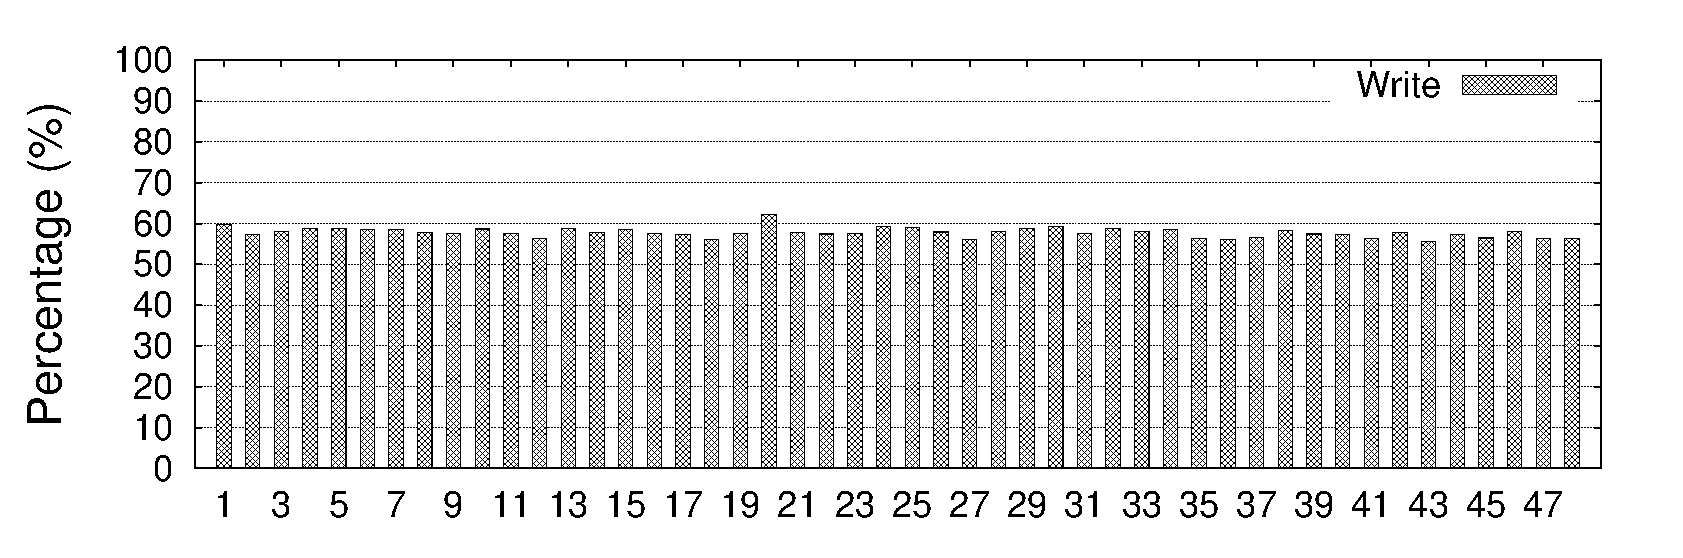
\includegraphics[width=0.5\textwidth]{./figs/spider1-rd-wr-ratio.eps}
%\includegraphics[width=0.5\textwidth]{}
\vspace{-0.1in}
\centering
\caption{Spider - Read Write Ratio}
\label{fig:rwratio}
\end{figure}


\subsection{I/O Requests}
\subsubsection{Request Size distribution}

\begin{figure}[!t]
\centering
\begin{tabular}{cc}
{\includegraphics[width=0.24\textwidth]{./figs/spider1-reqSizeCDF.eps}}&
{\includegraphics[width=0.24\textwidth]{./figs/spider1-reqSizePDF.eps}}\\
\end{tabular}
\vspace{-0.1in}
\centering
\caption{Spider 1 - Request size distribution}
\label{fig:spider1-reqsizedist}
\end{figure}

\begin{figure}[!t]
\centering
\begin{tabular}{cc}
{\includegraphics[width=0.24\textwidth]{./figs/spider2-reqSizeCDF.eps}}&
{\includegraphics[width=0.24\textwidth]{./figs/spider2-reqSizePDF.eps}}\\
\end{tabular}
\vspace{-0.1in}
\centering
\caption{Spider 2 - Request size distribution}
\label{fig:spider1-reqsizedist}
\end{figure}



\subsubsection{Request Size Latency distribution}

\begin{figure}[!t]
\centering
\begin{tabular}{cc}
{\includegraphics[width=0.24\textwidth]{./figs/spider2-reqLatCDF.eps}}&
{\includegraphics[width=0.24\textwidth]{./figs/spider2-reqLatPDF.eps}}\\
\end{tabular}
\vspace{-0.1in}
\centering
\caption{Spider 2 - Request Service Latency distribution}
\label{fig:spider1-reqLat}
\end{figure}




\subsection{Request Size vs Bandwidth}

 
